\chapter{Introducción}
\label{chap:introducion}

%% Borra esta anotación que che fago no teu seguinte commit
{\color{red} Emilio:}
{\color{gray} Movínche este parágrafo fóra da Motivación, para que o
  modifiques/mellores e sirva como entradiña para este capítulo de
  Introdución, de forma que na motivación presentes xa directamente o
  que nos propoñemos, e antes (aquí) introduzas o tema a tratar con un
  ou dos parágrafos, como este que tes, pero que hai que pulir un
  pouco:
  \begin{itemize}
  \item Tenta usar unha linguaxe o máis natural posible, que non soe
    forzada. Ademais, as frases, canto máis simples, mellor.
  \item Presenta e enlaza ben as ideas: no que dis, engade unha idea
    do que é a imaxe médica (como fas no resumo) e logo enlazas co
    tema da AR como un bo complemento nese eido, un pouco como o que
    temos no primeiro parágrafo do anteproxecto.
  \item Tenta fuxir dunha linguaxe excesivamente comercial,
    minimizando adxectivos que soan a `ventas', como aquí o de
    ``respuesta sólida''.
  \item Fíxate no {\tt .tex} en como poño as aspas/comillas, tanto as
    simples como as dobres, que é o xeito normal de facelo en \LaTeX.
  \end{itemize}
}
%% Borra o anterior ata aquí

\lettrine{D}{ebido} a los continuos avances en la tomografía computerizada, y en la medicina misma, las técnicas para reproducir estos conjuntos de datos, se han vuelto más y más importantes en los últimos 30 años como indica \cite{Botha2014}. En procura de estos nuevos métodos, se han establecido numerosos precedentes de la aplicación de la realidad aumentada en la medicina \cite{Sielhorst2008} ya que es posible su implementación en gran cantidad de tareas del sistema sanitario. Desde divulgación científica hasta cirugía guiada por imagen, la realidad extendida \footnote{Compendio de realidad virtual, realidad aumentada y realidad mixta.} se presenta como una respuesta sólida ante los problemas que acarrea la representación de información del ámbito médico.


\subsection{Motivación}

%% Borra esta anotación que che fago no teu seguinte commit
{\color{red} Emilio:}
{\color{gray} Escribe como motivación un texto parecido ao que temos
  no anteproxecto en 'breve descrición', un pouco máis elaborado (pero
  tampouco moito), e descartando o primeiro parágrafo que quizais
  encaixaría máis para o que comento arriba, para presentar o tema
  antes de comezar coa motivación. Non pasa nada se queda un chisco
  redundante cos obxectivos, que veñen despois. Aquí a idea é que
  quede máis «redactado» que é o que queremos facer, e tamén incluíndo
  o por que o queremos facer, mentres que os obxectivos son máis
  concretos e pormenorizados.
}
%% Borra o anterior ata aquí

\subsection{Objetivos}
Los objetivos principales de este proyecto son:
\begin{itemize}
    \item Analizar y diseñar marcas o guías a partir de imágenes capturadas mediante \acrfull{tc} para su impresión 3D, de forma que faciliten posteriormente el registro y seguimiento en 3D de los datos contenidos en la \acrshort{tc}.

%% Borra esta anotación que che fago no teu seguinte commit
{\color{red} Emilio:}
{\color{gray} A min quédame confuso este primeiro obxectivo (si, xa
  sei que o temos así literalmente no anteproxecto\ldots).  Eu poría
  primeiro quizais primeiro un obxectivo de extraer un modelo 3D a
  partir dun TC, e logo o de analizar e deseñar marcas ou guías para
  ser impresas tamén en 3D e facilitar o rexistro e seguimento e
  blabla.
}
%% Borra o anterior ata aquí

    \item Hacer detección, seguimiento y alineamiento 3D de la pieza impresa o guía en el flujo de vídeo capturado por un sistema de realidad aumentada, como puede ser un \acrshort{hmd} que incorpore cámaras de vídeo.
    \item Integrar elementos sintéticos en la imagen real de la visualización 3D.
    \item El objetivo final es disponer de un software capaz de resolver el problema del seguimiento y la estimación de pose en 3D y que pueda ser fácilmente integrable en un sistema de realidad Extendida completo
\end{itemize}

\subsection{Estructura de la memoria}

TODO

\subsection{Trabajo Previo}

%% Borra esta anotación que che fago no teu seguinte commit
{\color{red} Emilio:}
{\color{gray} Todo isto iría ao capítulo de Estado del Arte, non?
  Este capítulo 1, que habitualmente é un dos máis curtos da memoria,
  concluiría coa descrición da estrutura da memoria, que xa faremos
  cando teñamos máis ou menos todo escrito.
}
%% Borra o anterior ata aquí


\subsubsection{Visualización}
Los componentes artificiales que deseamos incluir en las imágenes del mundo real proceden del framework desarrollado por \citeauthor{Kroes2012} que aplica técnicas de \acrfull{mcrt} sobre \acrfull{dvr}.
\paragraph{}
El termino \acrshort{dvr} se utiliza para referirse a las técnicas que producen una imagen directamente a partir de datos de un volumen, sin realizar pasos intermedios. Para que esto sea posible es necesario implementar modelos físicos que indiquen cómo se genera, refleja, dispersa o oculta la luz \cite{Max1995}. Estos modelos con el paso del tiempo han evolucionado en modelos más y más complejos que han probado ser beneficiosos para la visualización científica de modelos 3D \cite{Daz2015}, \cite{Englund2016}, \cite{Lindemann2011} .

\paragraph{}
La implementación de estos modelos conlleva altos tiempos de renderizado, o en su defecto, un equipo increíblemente costoso para poder obtener una experiencia interactiva \cite{IglesiasGuitian2022}. Para enfrentar esta casuística,  \citeauthor{IglesiasGuitian2022} implementan un algoritmo de reducción de ruido basado en \acrfull{rls} que permite una experiencia interactiva en tiempo real, sobre \acrshort{gpu}s comerciales. Este proyecto se fundamenta en \cite{IglesiasGuitian2022} para el renderizado de las imágenes que posteriormente se apliquen en realidad aumentada sobre las imágenes reales.

\subsubsection{Realidad Extendida}
En 1994 \citeauthor{Milgram1994ATO} describe la realidad extendida como un subconjunto de tecnologías de la \acrfull{vr} que incorporan la mezcla entre el mundo real y el mundo virtual. 
Dado que existen tantas connotaciones y matices de realidad, \citeauthor{Milgram1994ATO} acuña el término de \textbf{\textit{virtuality continuum}}.
\paragraph{}
Este concepto de virtuality continuum \ref{fig:vc}, se caracteriza por comprender desde un usuario completamente inmerso en un mundo sintético que se comporta con algunas de las propiedades físicas del mundo real (incluso desafiando conceptos como la gravedad el tiempo o el espacio), hasta un usuario experimentando el mundo real con elementos virtuales añadidos o superpuestos.
Existen 4 conceptos bien diferenciados dentro del virtuality continuum:
\begin{itemize}
    \item Entorno Real (Real Enviroment): Consiste únicamente en objetos reales, situado al extremo izquierdo de \ref{fig:vc}.
    \item Realidad Aumentda(Augmented Reality): Mundo real aumentado o compuesto por elementos digitales.
    \item Virtualidad Aumentada(Augmented Virtuality): Mundo digital aumentado por objetos reales o fisicos.
    \item (Virtual Enviroment): Entorno puramente virtual.
\end{itemize}

\begin{figure}[hp!]
  \centering
  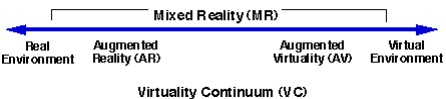
\includegraphics[width=0.75\textwidth]{imaxes/virtuality_continuum.png}
  \caption{Representacion simplificada de un virtuality continuum.}
  \label{fig:vc}
\end{figure}



Posteriormente \citeauthor{Azuma1997} definía la realidad aumentada como una variación de la realidad virtual, en la cual el usuario es capaz de ver el mundo real, con objetos virtuales superpuestos, o compuestos por el mundo real. La posibilidad de crear objetos y prototipos de forma rápida, sobre los cuales poder iterar y componer imágenes virtuales, demuestra el potencial de estas tecnologías trabajando a la par.
\paragraph{}

Para llevar a cabo el proyecto existen varias aproximaciones en el estado del arte \cite{Venkatesan2021}, así que se seleccionaron aquellas que más se ajustaban al proyecto.

--Discutir Aproximaciones--

Uno de los objetivos principales es el seguimiento de piezas extraídas de un \acrshort{tc} y diseñar marcadores que facilitasen el registro de las mismas, por lo que se optó por un seguimiento basado en marcadores. No obstante, en lo que a la visualización se refiere, es necesario un equipo con gran potencia computacional, o en su defecto, un visor que permita la reproducción de vídeo renderizado por un tercer equipo. Dadas estas restricciones se decidió por utilizar un \acrfull{hmd} HTC VIVE PRO. Utilizando \ref{fig:vrAproximations} como referencia, el sistema implementado se compondría de un seguimiento basado en marcadores (E) visualizando estos marcadores en realidad aumentada (B).


Para este proyecto se escogieron las tecnologías E y G que se observan en \ref{fig:vrAproximations}

\begin{figure}[hp!]
  \centering
  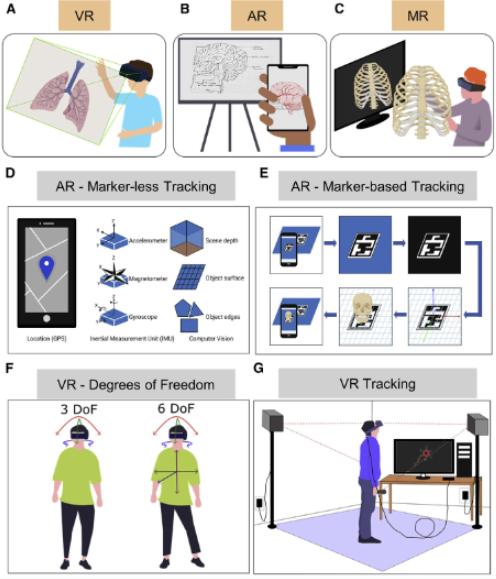
\includegraphics[width=0.75\textwidth]{imaxes/aproxVR.png}
  \caption{Aproximaciones a la realidad extendida para aplicaciones biomédicas.}
  \label{fig:vrAproximations}
\end{figure}


\subsubsection{Impresión 3D}
La impresión 3D o fabricación aditiva es un proceso para manufacturar objetos de cualquier forma o tamaño a partir de un modelo 3D o otro tipo de fuente electrónica a partir de procesos aditivos en los que sucesivas capas de material se depositan bajo control de un ordenador \cite{yan_dong_su_han_song_wei_shi_2018}.
Desde 1984 \cite{ChanaRodrguez2016} hasta la actualidad, la impresión 3D ha afrontado una revolución que se fundamenta en pilares sólidos como el abaratamiento de los costes de producción de impresoras 3D, la mejora de su precisión y velocidad, el software libre, la comercialización de los productos a usuarios finales , documentación, formación extensa corroborada y creada por terceros que facilita y realimenta el desarrollo de nuevos proyectos.
Producto de esto, ha sido la implementación de esta tecnología en el ámbito sanitario, tanto para la producción de herramientas especializadas \cite{ChanaRodrguez2016} como para el diseño y la implantación de prótesis personalizadas para cada paciente \cite{Gonzalez_Alvarez_2021}.



